% Drawing 138/06-13 -- folder 138, batch 06, archive page 108 (PDF page 109).
% Transcription: au crayon : une sphère (ellipse) portant un segment de $0$ à $1$ et un point $\infty$ ; un polygone à sept ou huit côtés découpé en secteurs par des rayons issus du centre.
% Kind: sphere with a segment; polygon cut into sectors (pencil). Method 2 (schematic redraw from the facsimile). Status: ok.
% Notes: Pencil. A sphere (ellipse) carrying the segment from 0 to 1 (inked) and the point infinity at the top; a polygon with seven sides (the transcription says seven or eight) cut into sectors by rays from the centre. Vertex positions approximate. The formulas across the middle are text.
% Coordinates: 1 unit = 1 mm = 1/100 of the crop width (bbox in page fractions: [0.132, 0.48, 0.88, 0.658]).
% Redrawn by Claude (claude-opus-5-5), issue #73, 2026-11-07; not checked by a human; not compiled (no TeX in the session).
% Rights: reproduces part of the work -- behind RENDER_TRANSCRIPTS, never published by itself.
\documentclass[tikz,border=3pt]{standalone}
\usepackage{amsmath,amssymb}
\usetikzlibrary{patterns,arrows.meta}
\tikzset{pencil/.style={black!45}, struck/.style={black!35}, mark/.style={circle,draw,inner sep=1.3pt}, pt/.style={circle,fill,inner sep=0.9pt}, opt/.style={circle,draw,fill=white,inner sep=1.1pt}}
\begin{document}
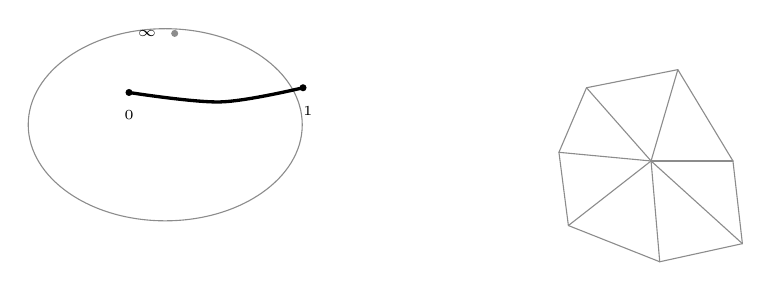
\begin{tikzpicture}[x=1mm,y=1mm,line cap=round,line join=round,font=\scriptsize]
\draw[pencil] (20.9,-12.8) ellipse[x radius=17.4, y radius=12.2];
\draw[very thick] plot[smooth, tension=0.55] coordinates {(16.3,-8.7) (27.9,-9.9) (38.4,-8.1)};
\node[pt] at (16.3,-8.7) {};
\node[pt] at (38.4,-8.1) {};
\node[inner sep=1pt] at (16.3,-11.6) {\tiny $0$};
\node[inner sep=1pt] at (39,-11) {\tiny $1$};
\node[pt,pencil] at (22.1,-1.2) {};
\node[inner sep=1pt] at (18.6,-1.2) {\tiny $\infty$};
\draw[pencil] (74.4,-8.1) -- (86,-5.8) -- (93,-17.4) -- (94.2,-27.9) -- (83.7,-30.2) -- (72.1,-25.6) -- (70.9,-16.3) -- cycle;
\draw[pencil] (82.6,-17.4) -- (74.4,-8.1);
\draw[pencil] (82.6,-17.4) -- (86,-5.8);
\draw[pencil] (82.6,-17.4) -- (93,-17.4);
\draw[pencil] (82.6,-17.4) -- (94.2,-27.9);
\draw[pencil] (82.6,-17.4) -- (83.7,-30.2);
\draw[pencil] (82.6,-17.4) -- (72.1,-25.6);
\draw[pencil] (82.6,-17.4) -- (70.9,-16.3);
\end{tikzpicture}
\end{document}
